% "{'classe':('PSI'),'chapitre':'stat_pfs_2d','type':('td'),'titre':'Chasse neige', 'source':'D\\'après documents Mines-Telecom.','comp':('B2-14','C1-05','C2-07'),'corrige':False}"
\setchapterimage{fig_02}
\chapter*{TD \arabic{cptTD} :
Chasse neige \ifnormal $\star$ \else \fi \ifdifficile $\star\star$ \else \fi \iftdifficile $\star\star\star$ \else \fi
 -- \ifprof Corrigé \else Sujet \fi}
\addcontentsline{toc}{section}{TD \arabic{cptTD} : 
Chasse neige \ifnormal $\star$ \else \fi \ifdifficile $\star\star$ \else \fi \iftdifficile $\star\star\star$ \else \fi
 -- \ifprof Corrigé \else Sujet \fi}

\iflivret \stepcounter{cptTD} \else
\ifprof  \stepcounter{cptTD} \else \fi
\fi

\setcounter{question}{0}
\marginnote{D'après documents Mines-Telecom.}
\marginnote{
\UPSTIcompetence[2]{B2-14}
\UPSTIcompetence[2]{C1-05}
\UPSTIcompetence[2]{C2-07}
}

%\begin{marginfigure}
%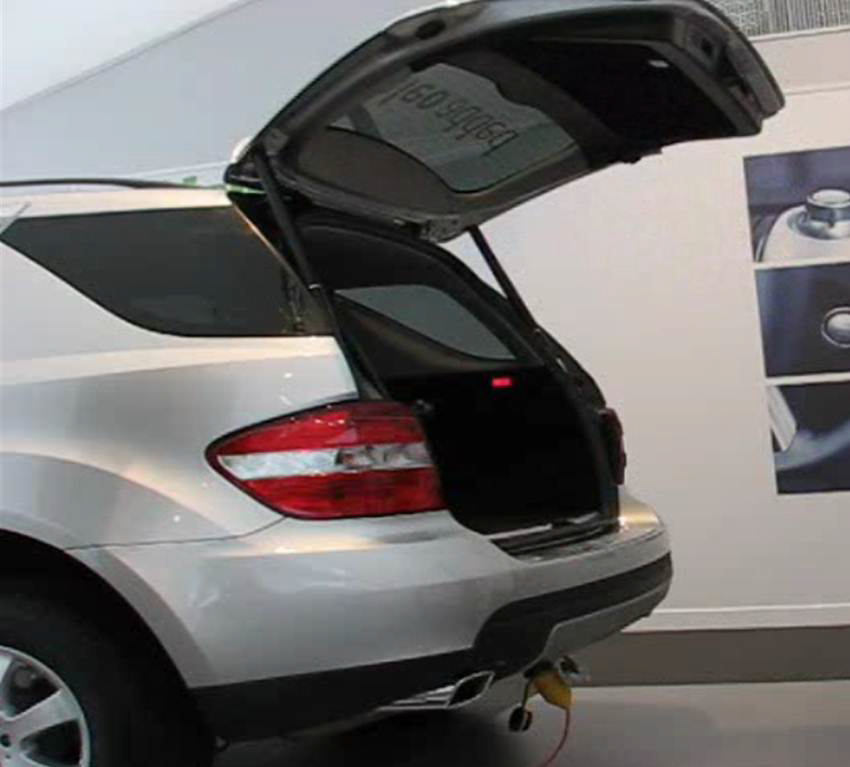
\includegraphics[width=\linewidth]{fig_00}
%\end{marginfigure}


\subsection*{Mise en situation}
\ifprof
\else
L’étrave de déneigement, objet de cette étude, est utilisée pour dégager les routes. Elle est composée de deux volets disposés en « V » qui permettent d’évacuer sur les côtés une épaisseur importante de neige. Les deux volets sont articulés de façon indépendante sur la pointe de l’étrave et ont une ouverture variable contrôlée par le conducteur à travers un vérin d’ouverture. En fin d’utilisation ou pour éviter des obstacles, elle est pourvue d’un système de relevage hydraulique.

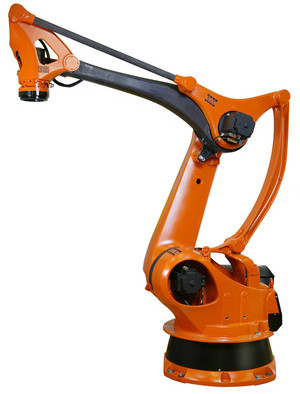
\includegraphics[width=\linewidth]{fig_01}

La pièce 7 est la lame de déneigement articulée par
rapport au châssis 3. Elle est mise en mouvement
par le vérin \{10 ; 11\}.



\subsection*{Données et hypothèses}
\begin{itemize}
\item $\gamma = \angl{x_3}{x_7}=\angl{z_3}{z_7}$ et $\beta= \angl{x_3}{x_{11}}=\angl{z_3}{z_{11}}$;
\item $\vect{z_{11}}=\vect{z_{10}}$ et $\vect{x_{11}}=\vect{x_{10}}$;
\item $\vect{HJ}=h\vect{z_7}$ et $\vect{HQ} = a\vx{3}+b\vy{3}+c\vz{3}$ et 
	$\vect{HG}=i\vect{z_7}$ et 
	$\vect{HM}=f\vect{x_3}+g\vz{3}$.
\end{itemize}

\begin{itemize}
\item Dans le cadre de cette étude, $\beta = 37\degres$ et $\gamma = 16\degres$, $\vect{g}=-g\vect{y_3}$;
\item liaisons parfaites (pas de jeu, pas de frottement);
\item le poids de toutes les pièces est négligé, sauf celui de la pièce 7, $m_7=\SI{850}{kg}$ appliqué en $G$;
\item dimensions en mètres :  $h=0,68$ ; $a=-0,33$ ; $b=0,1$; $c=1,1$ et $i=0,5$;
\item l’action de la neige sur le volet 7 est modélisée par un glisseur de moment nul en $Q$ tel que :
$\torseurstat{T}{\text{neige}}{7} =  \torseurl{Q\vx{7}}{\vect{0}}{Q}$ avec $Q = \SI{15000}{N}$;
\item le vérin d’ouverture choisi supporte une pression d'alimentation de 150 bars.
\end{itemize}

\fi
\subsection*{Problème ouvert}

\question{Proposer et mettre en \oe{}uvre une démarche permettant de déterminer la section du vérin permettant de « chasser la neige ». }

\subsection*{Problème décomposé}


\question{Réaliser les figures planes associées au paramétrage du problème.}

\question{Tracer le graphe de liaisons.}

\question{Déterminer la direction $\vect{u}$ de l'action mécanique $\vectf{11}{7}= F\vect{u}$.}

\question{En isolant 7, exprimer la relation liant $F$, $Q$ et les grandeurs géométriques.}

\question{En déduire la séction minimale $S$, du vérin permettant de chasser la neige.}

\ifprof
\else
\begin{marginfigure}
\begin{solution}
$S= - \dfrac{Q\left( a\sin \gamma+c\cos\gamma \right)  }{p h \sin\left(\beta - \gamma\right)}$.
\end{solution}
\end{marginfigure}
\fi


\ifprof
\begin{corrige}
\paragraph*{Graphe de liaisons}

On commence par faire les figures planes puis le graphe de liaisons.
\begin{enumerate}
\item On cherche les solides ou les ensembles de solides soumis à 2 glisseurs . Le problème étant plan, les pivots dont l'axe est perpendiculaire au plan sont des glisseurs. \{10+11\} est un ensemble soumis à 2 glisseurs.
\item On isole ensuite 7 et on rélise un théorème du moment statique en $H$ suivant $\vy{3}$.
\end{enumerate}

\begin{center}
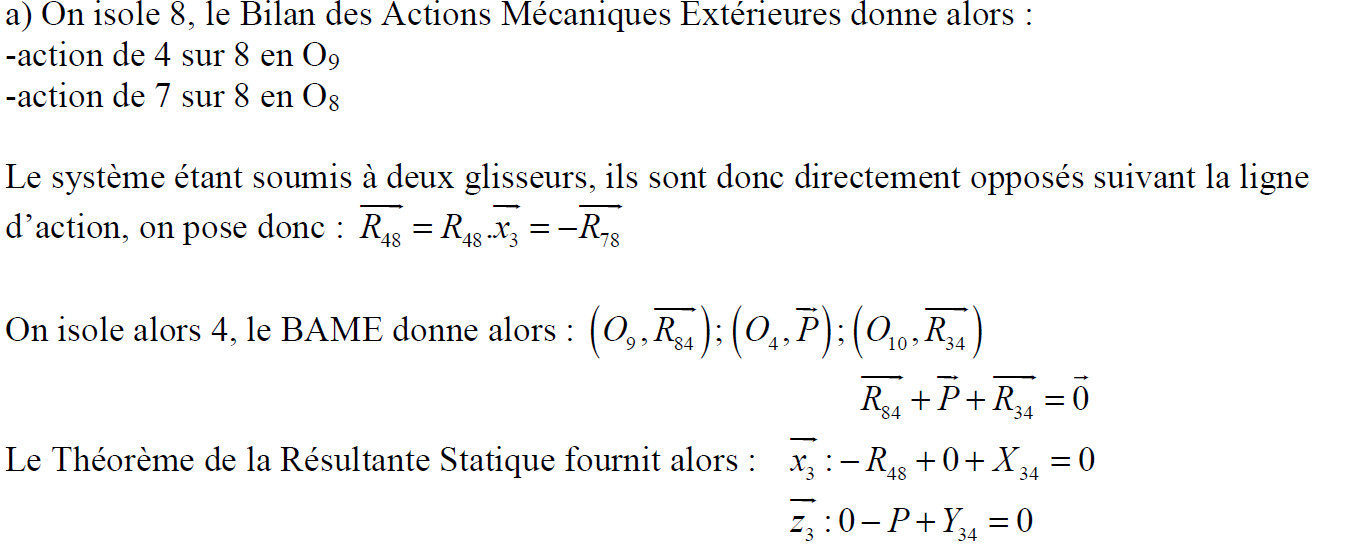
\includegraphics[width=\linewidth]{cor_01}
\end{center}

\paragraph*{On isole le vérin \{10+11\}}
D'après le PFS, l'ensmble étant soumis à 2 glisseurs, on a donc $\torseurstat{T}{11}{7} = \torseurl{F\vz{11}}{\vect{0}}{J}$.

\paragraph*{On isole \{7\}}
BAME : 
\begin{itemize}
\item action de la neige;
\item action de la pesanteur;
\item action de la pièce 11;
\item action de la pièce 3;
\end{itemize}

\paragraph*{On réalise le TMS en $H$ en projection sur $\vy{3}$.}

$$
\vectm{H}{\text{neige}}{7} \cdot \vy{3} + \vectm{H}{\text{Pesanteur}}{7} \cdot \vy{3} + \vectm{H}{11}{7} \cdot \vy{3} + \underbrace{\vectm{H}{3}{7} \cdot \vy{3}}_{\vect{0}} =0
$$

$
\Rightarrow
\left(\vect{HQ}\wedge Q\vect{x_7} \right) \cdot \vy{3} 
+ \left(\vect{HG}\wedge -gP\vect{y_3} \right) \cdot \vy{3} 
+ \left(\vect{HJ}\wedge F\vect{z_{11}} \right)  \cdot \vy{3}=0
$

$
\Rightarrow
\left(\left(a\vx{3}+b\vy{3}+c\vz{3}\right)\wedge Q\vect{x_7} \right) \cdot \vy{3} 
+ \underbrace{\left( i\vz{7}\wedge -gP\vect{y_3} \right) \cdot \vy{3}}_{\vect{0}}
+ \left(h\vz{7}\wedge F\vect{z_{11}} \right)  \cdot \vy{3}=0
$

$
\Rightarrow
\left(\vy{3} \wedge \left(a\vx{3}+c\vz{3}\right)  \right) \cdot   Q\vect{x_7}
+ \left(h\vz{7}\wedge F\vect{z_{11}} \right)  \cdot \vy{3}=0
$
$
\Rightarrow
\left( -a\vz{3}+c\vx{3}\right)   \cdot   Q\vect{x_7}
+ hF \sin\left(\beta - \gamma\right)\vy{3}  \cdot \vy{3}=0
$
$
\Rightarrow
Q\left( a\sin \gamma+c\cos\gamma \right)  
+ hF \sin\left(\beta - \gamma\right)=0
$

Au final, $F= - \dfrac{Q\left( a\sin \gamma+c\cos\gamma \right)  }{ h \sin\left(\beta - \gamma\right)}$.

$F$ étant l'effort déployé par le vérin, et $S$ sa section, on a alors, $F=pS$ et 
$S= - \dfrac{Q\left( a\sin \gamma+c\cos\gamma \right)  }{p h \sin\left(\beta - \gamma\right)}$.

\end{corrige}
\else
\fi